\documentclass[12pt]{article}
\usepackage{graphicx}
\usepackage{xcolor}
\usepackage{hyperref}
\usepackage{afterpage}
\definecolor{camerinoRed}{rgb}{.8,0,0}
\definecolor{camerinoBlue}{rgb}{.1,.23,.36}
\hypersetup{
    colorlinks=true, %set true if you want colored links
    linktoc=all,     %set to all if you want both sections and subsections linked
    linkcolor=blue,  %choose some color if you want links to stand out
}

\begin{document}
\pagestyle{empty}
\pagecolor{camerinoRed}
\begin{large}
\begin{center}
\begin{figure}
\centering
\includegraphics[scale=1]{knn.png}
\end{figure}
\textbf{\textcolor{black}{\uppercase{Distributed Calculus and Coordination}}}
\end{center}
\end{large}
\begin{normalsize}
\begin{center}
\textbf{\textcolor{black}{\uppercase{University of Camerino}}}

\textbf{\textcolor{black}{\uppercase{Faculty of Science and Technology}}}
\end{center}
\end{normalsize}

\vspace{3cm}


\begin{Huge}
\begin{center}
\textbf{\textit{\textcolor{white}{The Spy Game}}}
\end{center}
\end{Huge}


\vfill
\begin{tabbing}
 \hspace{11cm}\=\kill
  \textcolor{camerinoBlue}{\textbf{Made By:}} \> \textcolor{camerinoBlue}{\textbf{Accepted By:}}
 \end{tabbing}  
 \begin{tabbing}
 \hspace{11cm}\=\kill
  \textcolor{white}{Joni Seraj} \> \textcolor{white}{Emanuela Merelli}
 \end{tabbing}
 \newpage 
 \pagecolor{white}
 \begin{Huge}
 \textbf{Abstract}
 \end{Huge}
 \vspace{1cm}
 
 \begin{normalsize}
This report is about the Spy Game, a real-time, puzzle game featuring the theme of espionage. You will play using the role of a spy, infiltrating enemy bases with the goal of hacking information out of their computer terminals. As you try to accomplish this, there will be NPCs acting as your obstacles.
\\
The project is done using the multi-agent programmable modeling environment called NetLogo 6.0. While this platform has it's limitations, it certainly provided the tools to make the creation of this game possible.
\\
In this report we shall see how the game system is modeled and we will discuss the reasons why it was modeled in that particular way. We will discuss the multi-agent interactions, the system state changes, the way the game works etc.
 \end{normalsize}

\newpage
\tableofcontents
\newpage
\pagestyle{plain}
\pagenumbering{arabic}
\setcounter{page}{1}
\section{The Spy Game Concept}
\begin{normalsize}
In the spy game, you play the role of a spy. The game consists of you playing through different levels, infiltrating enemy bases, where you will encounter enemies (civilians, advanced civilians, guards). The goal is to get to the computer terminal on each level and hack it.\\
The genres consisting in the game's theme of espionage, are \emph{puzzle}, \emph{real-time} and \emph{click-to-play}.
Going through levels, one has to essentially solve the puzzles the map creator will have chosen for him. Sometimes the puzzle will be strictly timed events, sometimes logic decisions will have to be made to make progress. In all, the type of puzzles the game can make use of, remains in the creativity of the map maker.\\
Real-time means that the for the game to progress, time has to continuous. This is not to be confused with pausing the game, which is possible. Pausing the game merely allows the player to stop the game at a certain point. For him to make any actual progress, he has to unpause.
Click-to-Play is a term used to describe games where only by using the mouse can progress be made. This is a model that was fairly common in the old days of flash gaming( old as in the 2003-2006 when flash games were popular). The only was to interact with the agents in the game, is through the use of the mouse.
\end{normalsize}
\section{Development Tools}
The only development tool used in the making of this project is the Netlogo 6.0 multi-agent programmable environment. This platform eased quite a few instances in development( such as not having to create algorithms for grouping objects, determining which one is closer to the targets etc) and made other parts more difficult( such as providing limitations on the world, types of agents one could use, chaining events etc). I also have to mention my inexperience with the platform before this project, so maybe some of the aspects that I mention as difficult could be on my end.
\newpage
\section{Tile World}
NetLogo 6.0 Tile World is the map the game uses. Tile World is kinda like a chessboard. Chessboards have squares where pieces are put. The Tile World has patches instead of squares and agents instead of pieces.\\
The TileWorld size is determined by four values  max-pxcor, min-pxcor, min-pycor and max-pycor. As their names suggest, they determine the size of the map. The width of the world is determined by: $$ width = max-pxcor - min-pxcor $$ 
The height of the map can be determined using the same logic.\\
Every level of the game is a representation of the map and as such they are programmable. However, the question is raised, how do we implement them?\\
An alternative is to simply hard-code them in. However doing so, we would lose versatility of the code. Creating new levels would be such a painful process.\\
Due to the above problems, a better solution is needed. That's where NetLogo's FileIO comes in handy. By choosing to save the levels in files, we not only make it easy to create new levels, but we also remove the necessity to change the code every time. Instead we create a procedure to read the levels.\\
Now that the code versatility is solved, another problem is encountered. To have a procedure be able to read all levels, there must be a standart level representation in file formats. So all levels could be expressed in a file format in which they would be readable.\\
In order to solve this problem, we have to determine what different levels have in common and what differs them from one another. Using such logic, we can clearly see that all levels have world width and height, a matrix like structure and agents in it. So by all means we can express a level as a matrix which has a size of width x height.\\
But how would we express the agents and their positions in it? First we need to know how many types of agents we have. Our game has 8 types of entities( patches and agents ):
\newpage
\begin{itemize}
\item 0-Floor
\item 1-Wall
\item 2-Semi-Wall
\item 3-Spy
\item 4-Civilian
\item 5-Advanced Civilian
\item 6-Guard
\item 7-Computer
\end{itemize}
The numbers on the side are the number representation of the entity in the matrix. By placing the representations in the appropriate places, we can define a level.\\
But there are also differences in the levels which we must consider. There is one that we must solve, guard patrols. Patrols will be different on different levels, as the structure of the map changes. So in order to define levels, we must define the behaviour of guards. We can do this by adding lines of commands as "up","down","right","left" and "stop". The first four are intuitive, while the fifth will be used to end a patrol definition, so to allow for custom guard placement in levels and custom guard patrols.\\
In the next page a tile world representation is shown in file format and game.
\begin{figure}
\centering
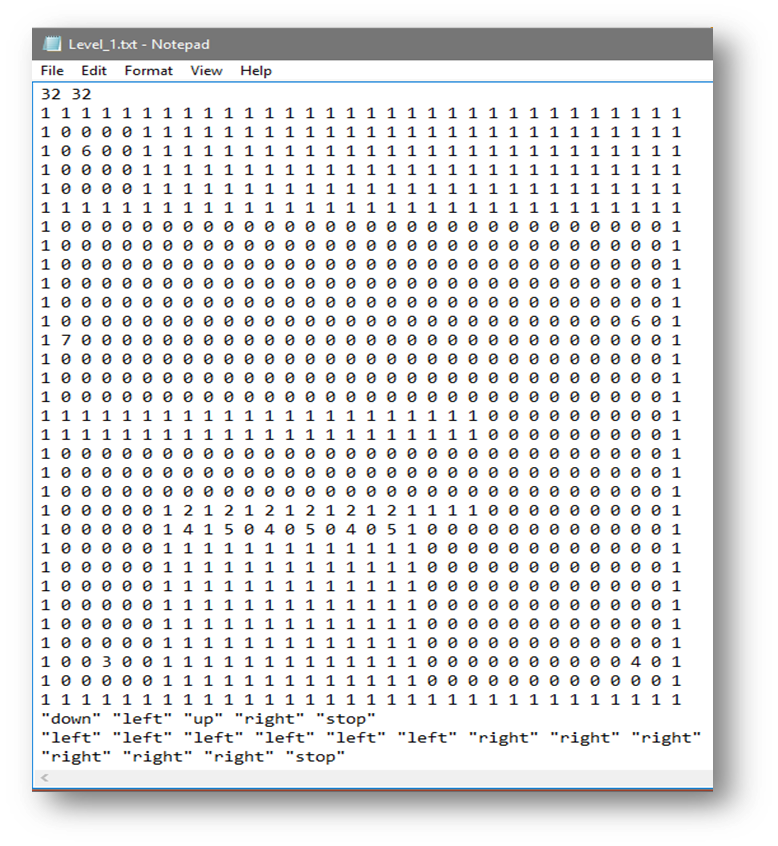
\includegraphics[scale=.7]{Picture2.png} 
\caption{File Format Representation}
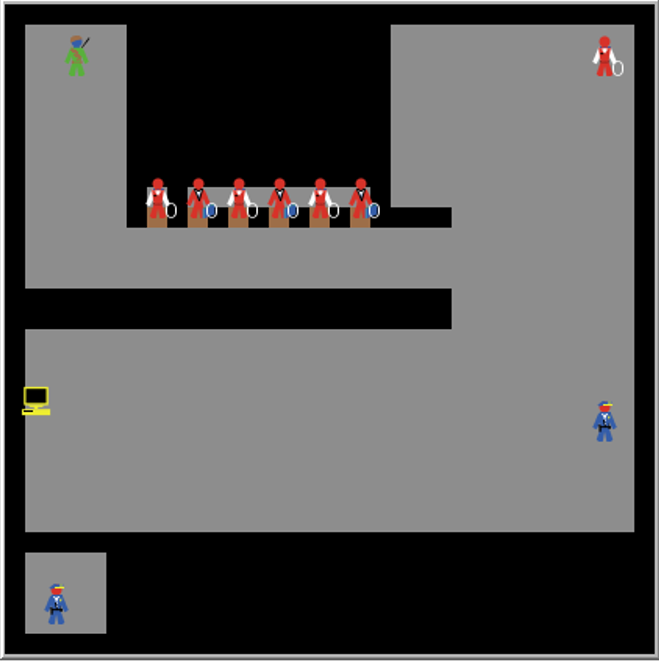
\includegraphics[scale=.5]{Picture3.png}
\caption{Game Representation}
\end{figure}
\newpage
\section{Initialization and Globals}
Initializing the game requires quite a couple of steps. In NetLogo, we do it through a procedure called setup, global variables and breeds.\\
\vspace{0.1cm}
Breeds are classes of agents. They can be turtles, can be patches etc. We use them to define classes for spies, civilians, advanced civilians, guards, computers and holos (simply used to make a game feature possible). After simply declaring the breeds, we define special properties these breeds will have. Civilians and Advanced Civilians will have the variable of suspicion. Guards will have the properties of patrolList( list of patrol commands ), originalX and originalY ( guards spawning coordinates), alerted (flag for movement), patrolNum ( used to keep track of patrol command position ).\\
\vspace{0.1cm}
After breed definitions, we need to declare our globals, variables that will be shared through all of the procedures. Important globals are alert ( if true, environment changes to a state of alarm, otherwise false), trigger ( true if an alarm has ocurred ), alertX and alertY ( last known coordinates of spy when in alarm mode ) and countdown which determines how long the state of alarm will last.\\
\vspace{0.1cm}
After the declaration of breeds and globals, we call the procedure of setup, which invokes the read file procedure, responsible for reading the level files and translating them into the world.\\
\vspace{0.1cm}
During these procedure the file is read, the world size is set and agents and patches are set properly. At this point, the game is ready to run.
\newpage
\section{Environment}
The environment can be represented as a set of three elements:
$$ Environment = <E,e0,t> $$
E is the set of all possible states of the system, e0 is the initial state while t is the state transition function.\\
Our game system can be interpreted as having 4 different states:
\begin{enumerate}
\item Game Lost
\item Game Won
\item Alarmed
\item Idle
\end{enumerate}
Idle is the default state, or the e0. Through the t function, the states change in between them. When an alarm happens, the system passes from Idle to Alarmed. When the spy hacks the computer terminal, system passes from Idle or Alarmed to Game Won. When the spy gets caught,  system passes from Idle or Alarmed to Game Lost.
\section{Agents}
The agents in the spy game are of 6 types:
\begin{itemize}
\item Observer (player)
\item Spy
\item Computer
\item Civilian
\item Advanced Civilian
\item Guard
\end{itemize}
\newpage
\subsection{Observer}
The observer is the player itself. He controls the game using the mouse. He has two different interactions with other agents:
\begin{itemize}
\item When the player holds down the mouse button on a floor, the spy tries to move it.
\item When he clicks an enemy unit, a civilian, an advanced civilian or a guard, the enemy unit is highlighted and it's detection radius is shown.
\end{itemize}
\vspace{3cm}
\begin{figure}[h]
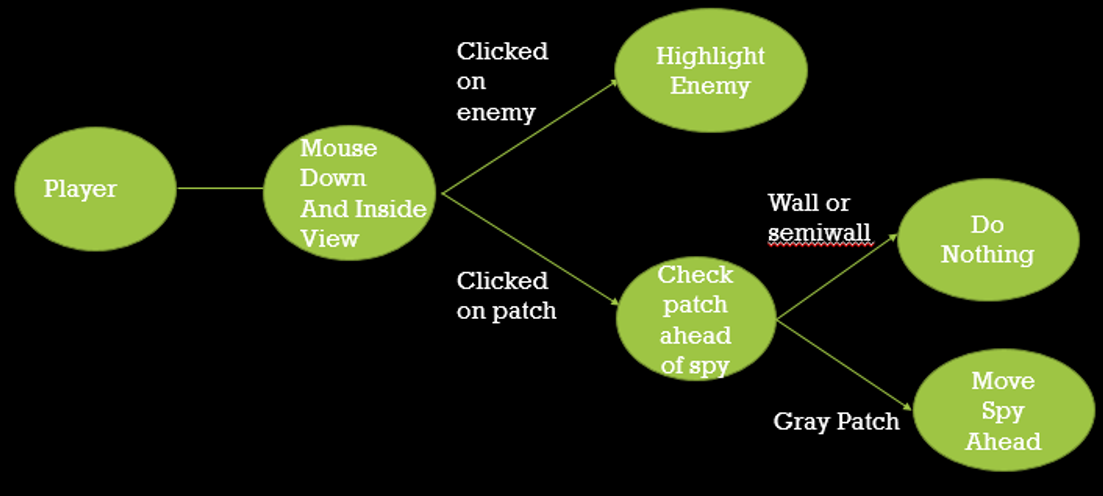
\includegraphics[scale=.8]{Picture4.png}
\caption{Action Tree of Player}
\centering
\end{figure}
\newpage
\subsection{Spy}
The spy is an agent whose actions are controlled by the player. Despite the previously stated fact, it's interactions with other agents are quite a few and important.
\begin{itemize}
\item When a patch away from the computer, game is won.
\item When entering guards radii of detection, game is lost.
\item When entering civilians radii of detection, raise their suspicion.
\item When exiting civilians radii of detection, lower their suspicion.
\item When entering advanced civilians radii of detection, raise their suspicion.
\end{itemize}
\subsection{Computer}
The computer is a stationary agent whose only purpose is it's interaction with the spy as mentioned above.
\newpage
\subsection{Civilian}
\begin{figure}[h]
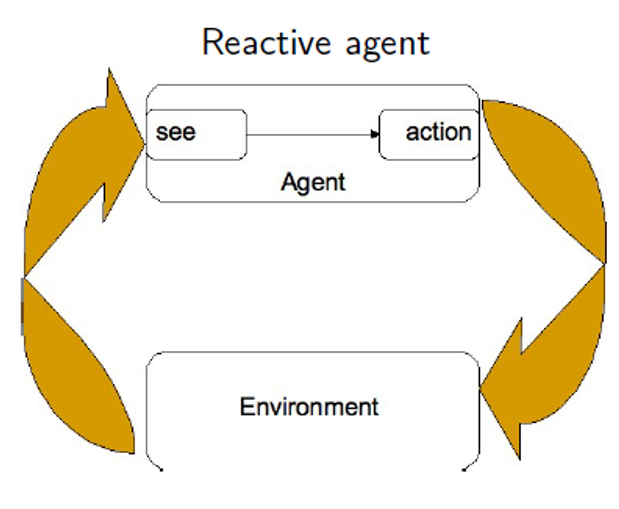
\includegraphics[scale=1]{Picture5.png}
\centering
\caption{Reactive agent way of functioning}
\end{figure}
Civilians are reactive agents. They react to the environment and are able to change it's state. As such, they do not possess any kind of memory of the previous states of the environment nor does it affect their behaviour.\\
Their interactions with other agents include:
\begin{itemize}
\item When spy enters their detection radii, they raise their suspicion level. If it reaches 100, guards all called and the environment is passed in an alarm state.

\item If spy is not in their detection radii and the environment is not in an alarm state their suspicion goes down with time.

\item Once in alarm state, if spy enters the detection radii, they report the new position of him.

\item When clicked by the player, it will show it’s detection radii.
\end{itemize}
\begin{figure}[p!]
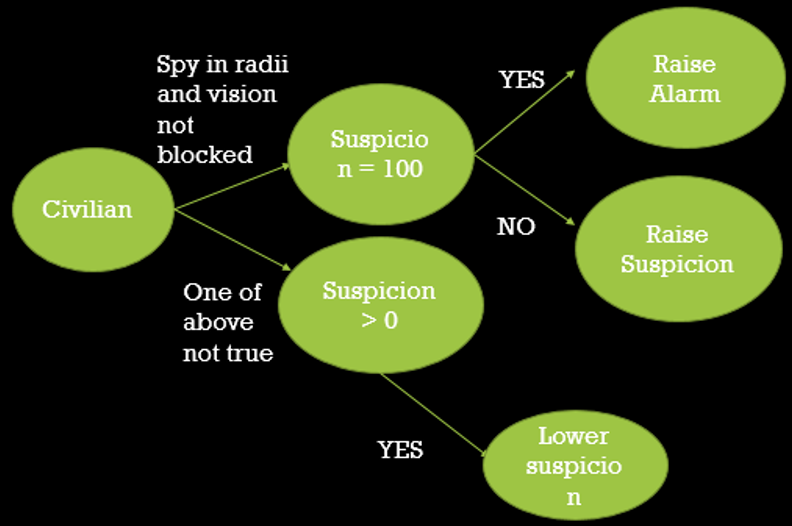
\includegraphics[scale=1]{Picture6.png}
\centering
\caption{Action tree of civilian agent}
\end{figure}
\newpage
\subsection{Advanced Civilian}
\begin{figure}[h]
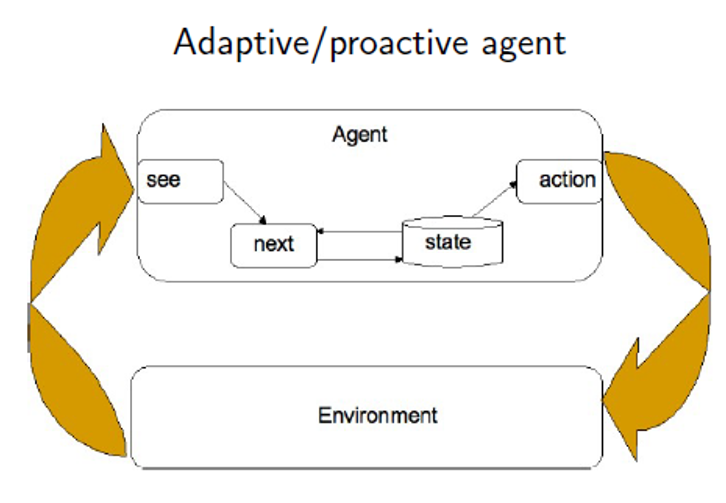
\includegraphics[scale=1]{Picture7.png}
\centering
\caption{Adaptive agent way of functioning}
\end{figure}
Advanced Civilians are adaptive agents. They react to the environment and are able to change it's state. They do possess memory of the previous states of the environment and it affect their behaviour. In difference to Civilians, Advanced Civilians do not lower their suspicion levels and once an alarm is raised, they will remain alarmed for the rest of the level.\\
Their interactions are the same as those of civilians.
\afterpage{
\begin{figure}[h]
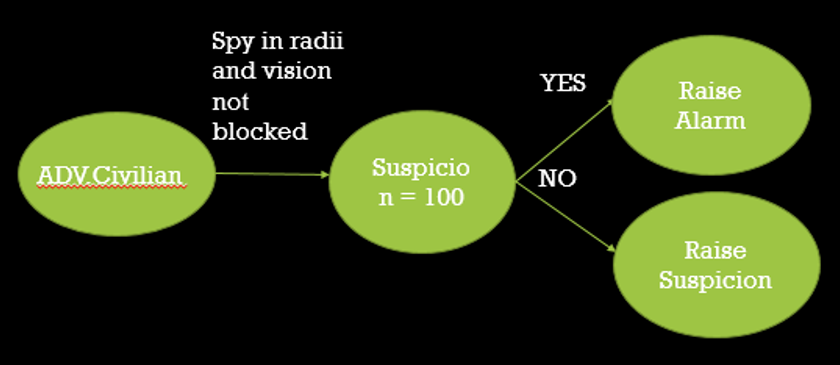
\includegraphics[scale=1]{Picture8.png}
\centering
\caption{Action tree of advanced civilian agent}
\end{figure}
\clearpage
}
\newpage
\subsection{Guard}
Guards are pro-active agents. They have different behaviours when in different environment states and internal states. Guards can be alerted or not alerted despite the system's alerted state. Only one guard can be alerted at a certain time and that is the one who is closer to the last known position of the player ( of course in an alarm environment state ). When not in an alarm state, guards follow their patrol lines. Their internal state is made possible by their property \emph{alerted}.\\
Guards have the following interactions:
\begin{itemize}
\item Guard detects spy, game is lost.
\item Alarm state is raised by civilians, if guard is the nearest to the last known position of the player goes and investigates.
\item When clicked, detection radii is shown.
\end{itemize}
\begin{figure}[h]
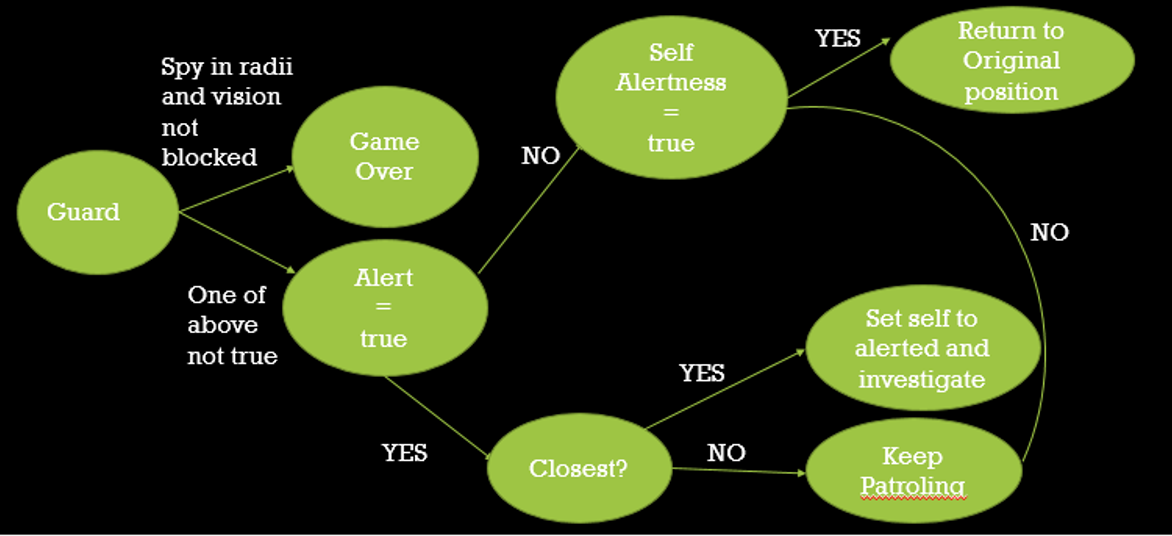
\includegraphics[scale=.7]{Picture9.png}
\centering
\caption{Action tree of guard agent}
\end{figure}
\newpage
\section{Rules}
\begin{itemize}
\item Walls are impassable by both movement and vision.
\item Half-Walls are impassable by movement but not vision.
\item Raising a civilians level of suspicion will evoke an alarm.
\item An alarm will make every enemy suspicious and during it’s time period, levels of suspicion will be all high. Afterwards, advanced civilians will keep their suspicion, civilians will start to lower it while guards will return to their posts.
\item The game will be lost immediately if entering field of view of a guard.
\item Levels can be won only by being a tile away from the computer.
\end{itemize}
\section{Summary and Conclusions}
The whole game is built using NetLogo, which provides the means for a system analyzed as a multi-agent environment model. It was for me an absolutely new experience, having to make my mind think in a different way, focusing more on the behaviour of the agents and the way it affected the system. This report provides such an analization of the spy game, which includes three different type of agents, reactive, adaptive, pro-active and explains how their interactions transition the environment through different states.
\newpage
\section{References}
\begin{itemize}
\item NetLogo Model Library
\item NetLogo User Manual
\item NetLogo Programming Guide
\item UNICAM DCC Lectures - Emanuela Merelli 2017
\end{itemize}
\vfill
\begin{Huge}
\begin{center}
\textbf{End of Report}\\
\textbf{Thank you for reading!}\\
\end{center}
\end{Huge}
\end{document}